\documentclass[12pt]{article}

\usepackage{sbc-template}
\usepackage{graphicx,url}
\usepackage[utf8]{inputenc}
\usepackage[brazil]{babel}
\usepackage{float}

\makeatletter
\renewenvironment{thebibliography}[1]
     {\section*{\refname
        \@mkboth{\MakeUppercase\refname}{\MakeUppercase\refname}}%
      \list{\@biblabel{\@arabic\c@enumiv}}%
           {\settowidth\labelwidth{\@biblabel{#1}}%
            \leftmargin\labelwidth
            \advance\leftmargin\labelsep
               \itemindent -\leftmargin
               \itemsep 1.5pt
            \@openbib@code
            \usecounter{enumiv}%
            \let\p@enumiv\@empty
            \renewcommand\theenumiv{\@arabic\c@enumiv}}%
      \sloppy
      \clubpenalty4000
      \@clubpenalty \clubpenalty
      \widowpenalty4000%
      \sfcode`\.\@m}
     {\def\@noitemerr
       {\@latex@warning{Empty `thebibliography' environment}}%
      \endlist}
\makeatother

\raggedbottom
\sloppy

\title{Mobilidade e Densidade em Redes Ad Hoc: uma Avaliação Estatística de AODV, OLSR e DSDV}

\author{Guilherme Alixandre Gonçalves Silva, Gabriel Araujo de Ataides, Victor Inacio}

\address{Instituto Federal de Educação, Ciência e Tecnologia de Goiás (IFG) -- Campus Inhumas\\
  Inhumas -- GO -- Brasil
  \email{\{guilherme.silva,g.ataides,victor.inacio\}@estudante.ifg.edu.br}
}

\begin{document}

\maketitle

\begin{resumo}
Trabalhos sobre MANETs costumam enquadrar a comparação de protocolos em torno da dicotomia reativo/proativo, tratando a densidade de nós como fator secundário. Apresentamos um estudo em ns-3 de AODV, OLSR e DSDV sob quatro velocidades de mobilidade (1--20~m/s) \emph{e} duas densidades de nós (20 e 10, na mesma área), com 60 repetições independentes por cenário e testes de hipótese não paramétricos (Kruskal-Wallis; Mann-Whitney com correção de Holm). O AODV empata com o OLSR em taxa de entrega (PDR), mas tem atraso e jitter significativamente maiores; ambos superam o DSDV em PDR. Mais surpreendente: reduzir a densidade pela metade \emph{melhora} significativamente o PDR do DSDV (seus broadcasts periódicos da tabela completa escalam com o número de nós) e \emph{piora} o atraso e o jitter do AODV (mais sobrecarga de descoberta de rota sob demanda por vizinho) -- a densidade prejudica ou beneficia cada protocolo por um mecanismo diferente, não uniformemente. Uma correção de reprodutibilidade nos fluxos de números aleatórios do simulador também é reportada.
\end{resumo}

\noindent\textbf{Palavras-chave:} MANET, roteamento \textit{ad hoc}, mobilidade, AODV, OLSR, DSDV, ns-3.

\section{Introdução}

Em comparações de protocolos de roteamento para MANET, é comum partir da expectativa de que um protocolo reativo como o AODV (\textit{Ad hoc On-Demand Distance Vector}) entrega mais pacotes que protocolos proativos como o OLSR (\textit{Optimized Link State Routing}) e o DSDV (\textit{Destination-Sequenced Distance-Vector}), em troca de maior atraso e jitter -- já que descobre rotas sob demanda e enfileira pacotes durante essa descoberta, em vez de descartá-los imediatamente. Menos discutido é o efeito da \emph{densidade} da rede: reduzir o número de nós na mesma área é, em geral, tratado como um prejuízo uniforme à conectividade -- mas será que afeta os três protocolos da mesma forma e pela mesma razão?

Para responder, comparamos os três protocolos em ns-3 sob quatro velocidades e duas densidades (20 e 10 nós, mesma área), validando as diferenças com testes não paramétricos.

Contribuições: (i) comparação experimental de AODV, OLSR e DSDV sob mobilidade variável, com validação estatística par-a-par; (ii) análise do efeito da densidade em cada protocolo, não uniforme nem sempre prejudicial, com explicação mecanística; e (iii) a correção de um problema de reprodutibilidade dos números pseudoaleatórios do simulador.

\section{Trabalhos Relacionados}

A literatura sobre comparação de protocolos MANET não é unânime. \cite{quadri2025} comparam AODV, OLSR e DSDV em ns-3 variando densidade, concluindo que o AODV obtém o maior PDR -- mas sem isolar o efeito da densidade por protocolo, feito aqui (Seção~\ref{sec:densidade}). \cite{arunkumar2008} e \cite{shrivastava2021} chegam a conclusões semelhantes em NS-2 e VANET. \cite{alkhatib2018} reportam vantagem do DSDV (proativo) sob mudanças de topologia -- retomado na Seção~\ref{sec:discussao}. \cite{alzahrani2020} relacionam os retransmissores multiponto do OLSR a menor sobrecarga de controle, base da explicação mecanística adotada aqui; \cite{almaliki2024} ligam instabilidade de topologia a maior atraso fim-a-fim. \cite{chrysoula2012} reforça que o comportamento relativo é sensível ao cenário -- o que motiva a validação estatística, não só visual, feita aqui.

\section{Metodologia}

O cenário foi simulado no ns-3 (versão 3.48) \cite{nsnam2024} com rede 802.11b \textit{ad hoc}, em área de $500\times500$~m, nós uniformemente distribuídos e movendo-se por RandomWaypoint (velocidade constante por rodada, pausa de 1~s). Quatro fluxos UDP determinísticos transmitem pacotes de 1024~bytes a cada 0,1~s, entre 15~s e 118~s de 120~s de simulação -- o atraso inicial dá tempo dos protocolos convergirem antes de medir. O experimento tem \emph{dois} estágios: 20 nós (base) e 10 (extensão), mesma área -- a variável de densidade deste trabalho.

Cada combinação de protocolo, velocidade e densidade foi repetida 60 vezes, com seed mestre fixa e \textit{run} variável -- o ns-3 salta entre substreams independentes do gerador MRG32k3a, garantindo repetições independentes e reprodutíveis -- 1440 execuções no total. As métricas -- PDR, throughput, atraso e jitter médios -- vêm do FlowMonitor do ns-3, agregadas por execução; atraso e jitter só contam pacotes recebidos, limitação retomada na Seção~\ref{sec:discussao}. Como essas duas têm cauda longa (Shapiro-Wilk por célula), usamos testes não paramétricos: Kruskal-Wallis entre os 3 protocolos por velocidade, e Mann-Whitney par-a-par -- entre protocolos, e entre as duas densidades por protocolo/velocidade --, com correção de Holm e tamanho de efeito pelo delta de Cliff. Médias e IC95\% são só resumo descritivo.

\textbf{Nota de reprodutibilidade.} Wi-Fi e roteamento não tinham fluxos pseudoaleatórios atribuídos via \texttt{AssignStreams}, ao contrário da mobilidade; como o contador global do ns-3 nunca era reiniciado entre as 1440 execuções, cada resultado dependia de quantas execuções vieram antes. Corrigido com \texttt{AssignStreams} explícito para Wi-Fi/roteamento mais \texttt{ResetNextStreamIndex()} por execução (o primeiro sozinho não bastava); os resultados aqui já refletem a correção. \textbf{Reprodutibilidade:} código, scripts de análise/gráficos, dados brutos e instruções completas de execução estão em \url{https://github.com/MrCode-Man/manet-ns3}.

\section{Resultados}

A Tabela~\ref{tab:resumo} resume as quatro métricas ($n=60$) por protocolo, velocidade \emph{e} densidade (colunas ``20''/``10''). A Figura~\ref{fig:pdr-jitter} mostra o mesmo em função da velocidade (cor = protocolo, sólido = 20 nós, tracejado = 10 nós).

\begin{table}[H]
\centering
\caption{Médias de PDR (\%), atraso (ms) e jitter (ms), $n=60$, nas duas densidades.}
\label{tab:resumo}
\scriptsize
\renewcommand{\arraystretch}{0.72}
\begin{tabular}{llrrrrrr}
\hline
 & & \multicolumn{2}{c}{\textbf{PDR (\%)}} & \multicolumn{2}{c}{\textbf{Atraso (ms)}} & \multicolumn{2}{c}{\textbf{Jitter (ms)}} \\
\textbf{Proto.} & \textbf{v} & 20 & 10 & 20 & 10 & 20 & 10 \\
\hline
AODV & 1  & 73,4 & 75,3 & 11,5 & 8,9  & 6,3 & 3,9 \\
AODV & 5  & 76,6 & 71,6 & 13,2 & 8,8  & 6,9 & 4,4 \\
AODV & 10 & 75,3 & 76,7 & 12,9 & 13,9 & 7,6 & 5,2 \\
AODV & 20 & 74,7 & 71,3 & 13,1 & 13,9 & 7,8 & 5,9 \\
OLSR & 1  & 74,7 & 74,3 & 6,6  & 6,6  & 3,0 & 2,9 \\
OLSR & 5  & 72,4 & 76,0 & 6,7  & 6,6  & 3,2 & 2,9 \\
OLSR & 10 & 74,9 & 68,7 & 7,7  & 7,0  & 3,9 & 3,3 \\
OLSR & 20 & 66,5 & 58,3 & 8,2  & 7,2  & 4,5 & 3,4 \\
DSDV & 1  & 56,9 & 71,5 & 6,4  & 6,4  & 2,9 & 2,7 \\
DSDV & 5  & 59,2 & 72,9 & 6,5  & 6,8  & 3,0 & 3,1 \\
DSDV & 10 & 52,7 & 65,8 & 6,1  & 6,6  & 2,9 & 3,1 \\
DSDV & 20 & 43,6 & 57,0 & 5,9  & 6,3  & 2,8 & 3,0 \\
\hline
\end{tabular}
\end{table}

\vspace{-9mm}
\begin{figure}[H]
\centering
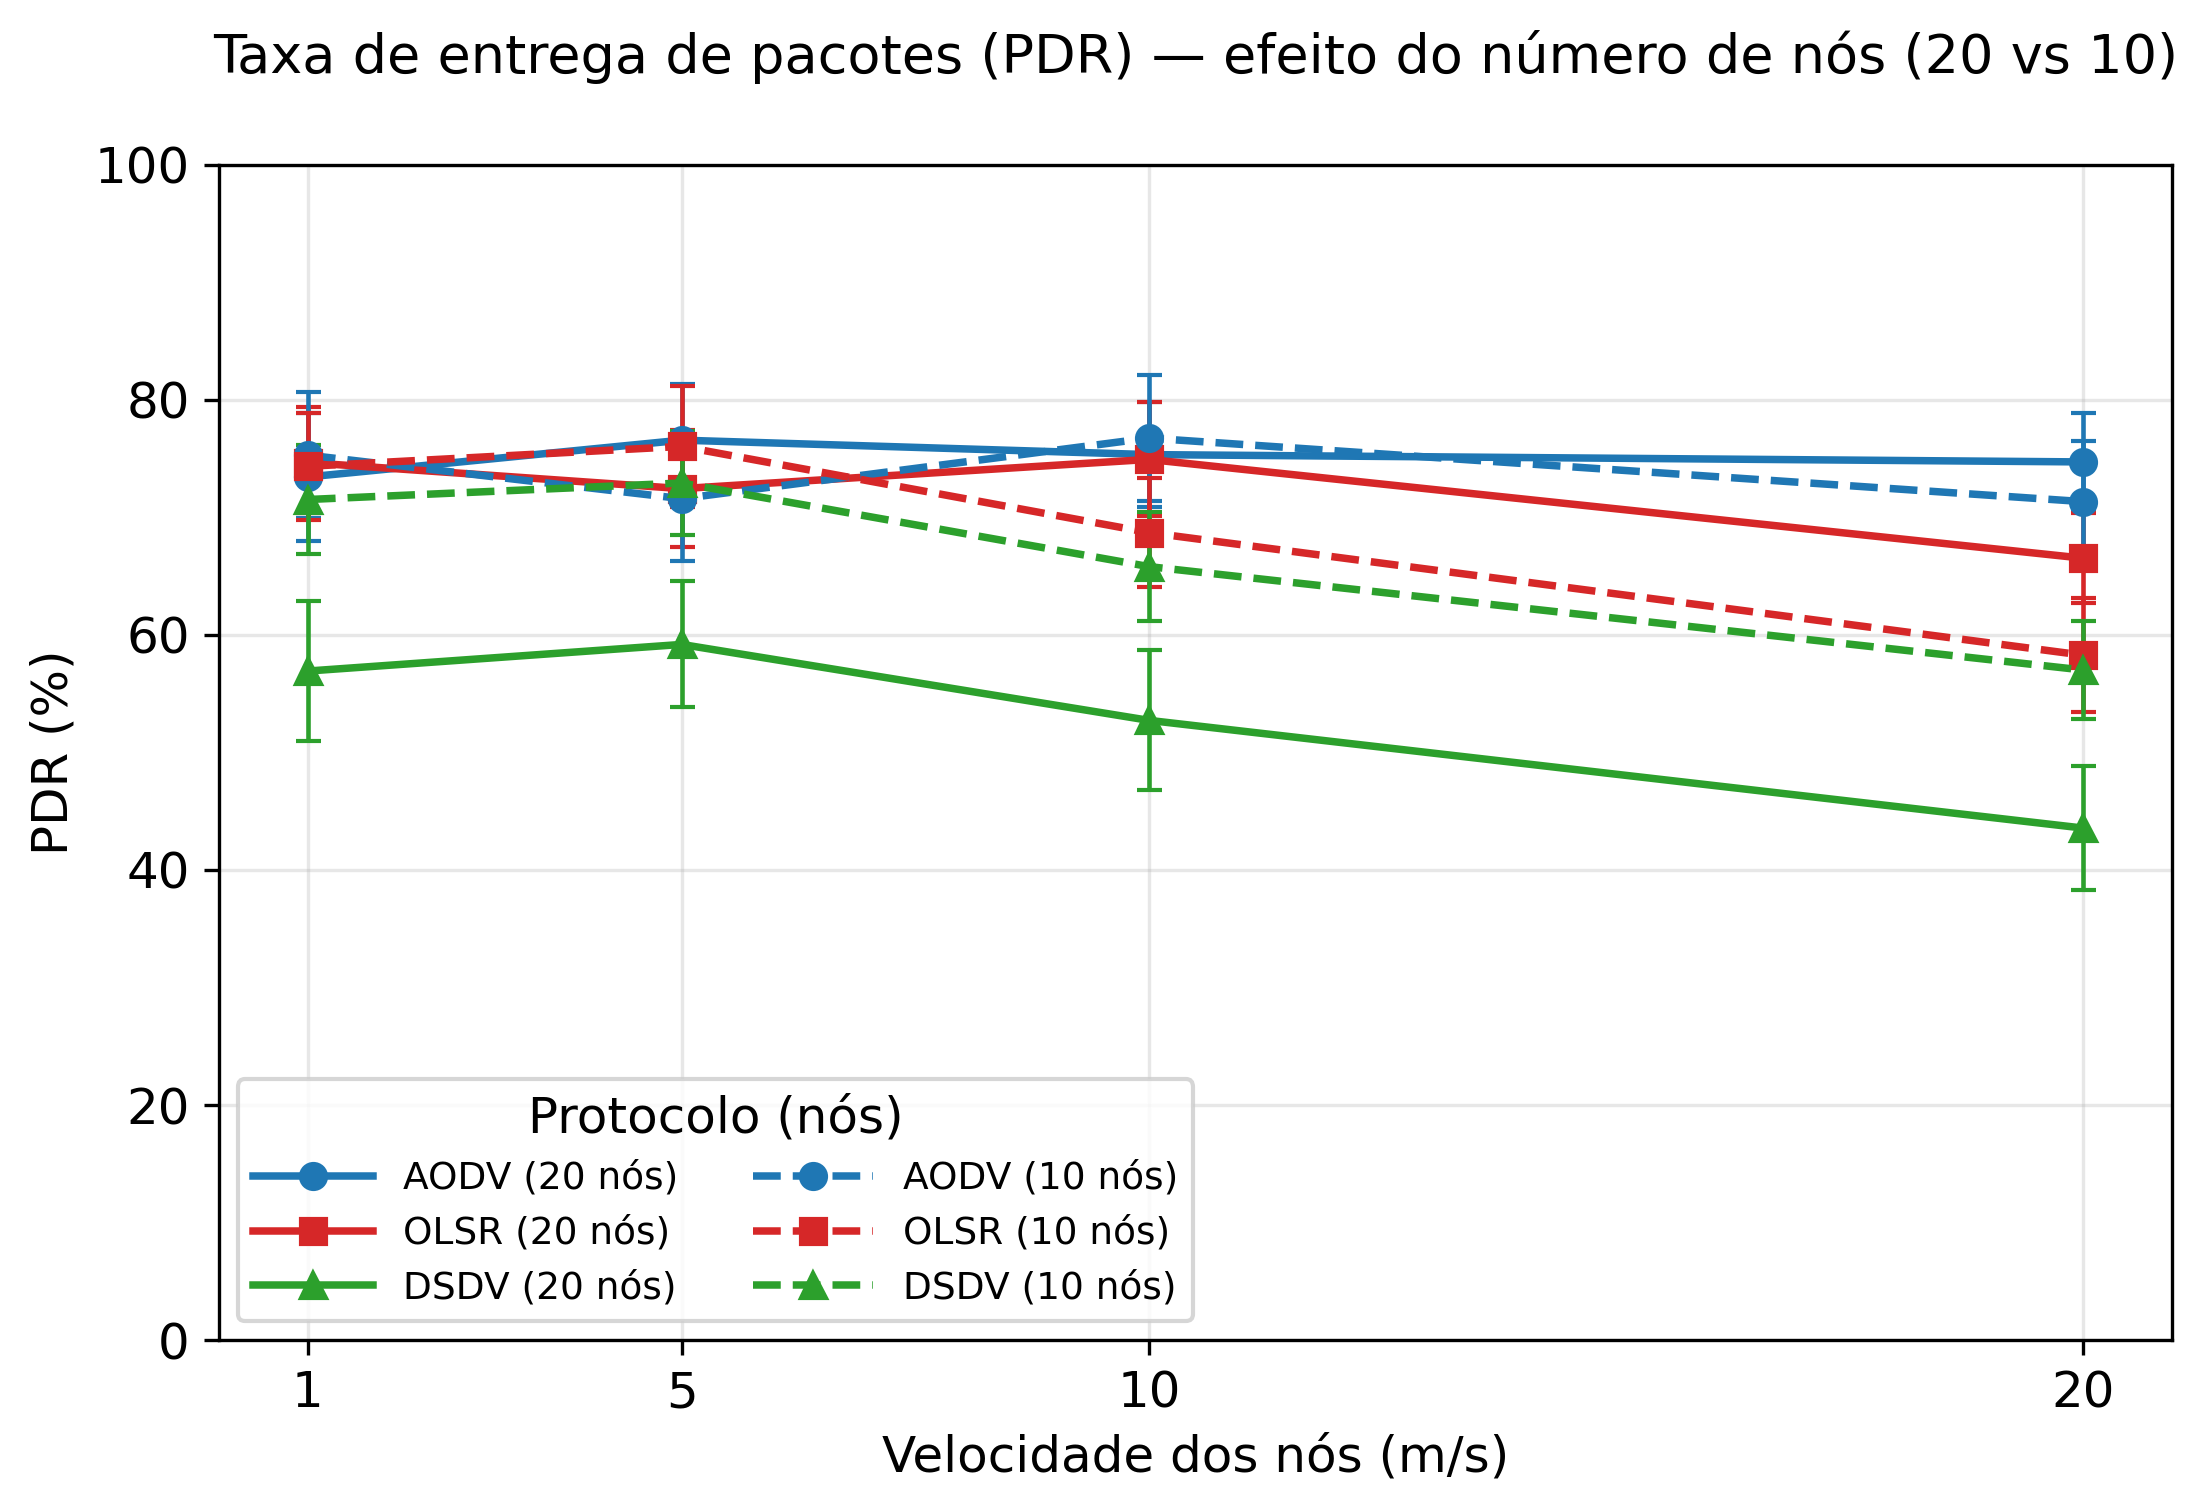
\includegraphics[width=.47\linewidth]{../figures/pdr_nodes_comparison.png}
\hfill
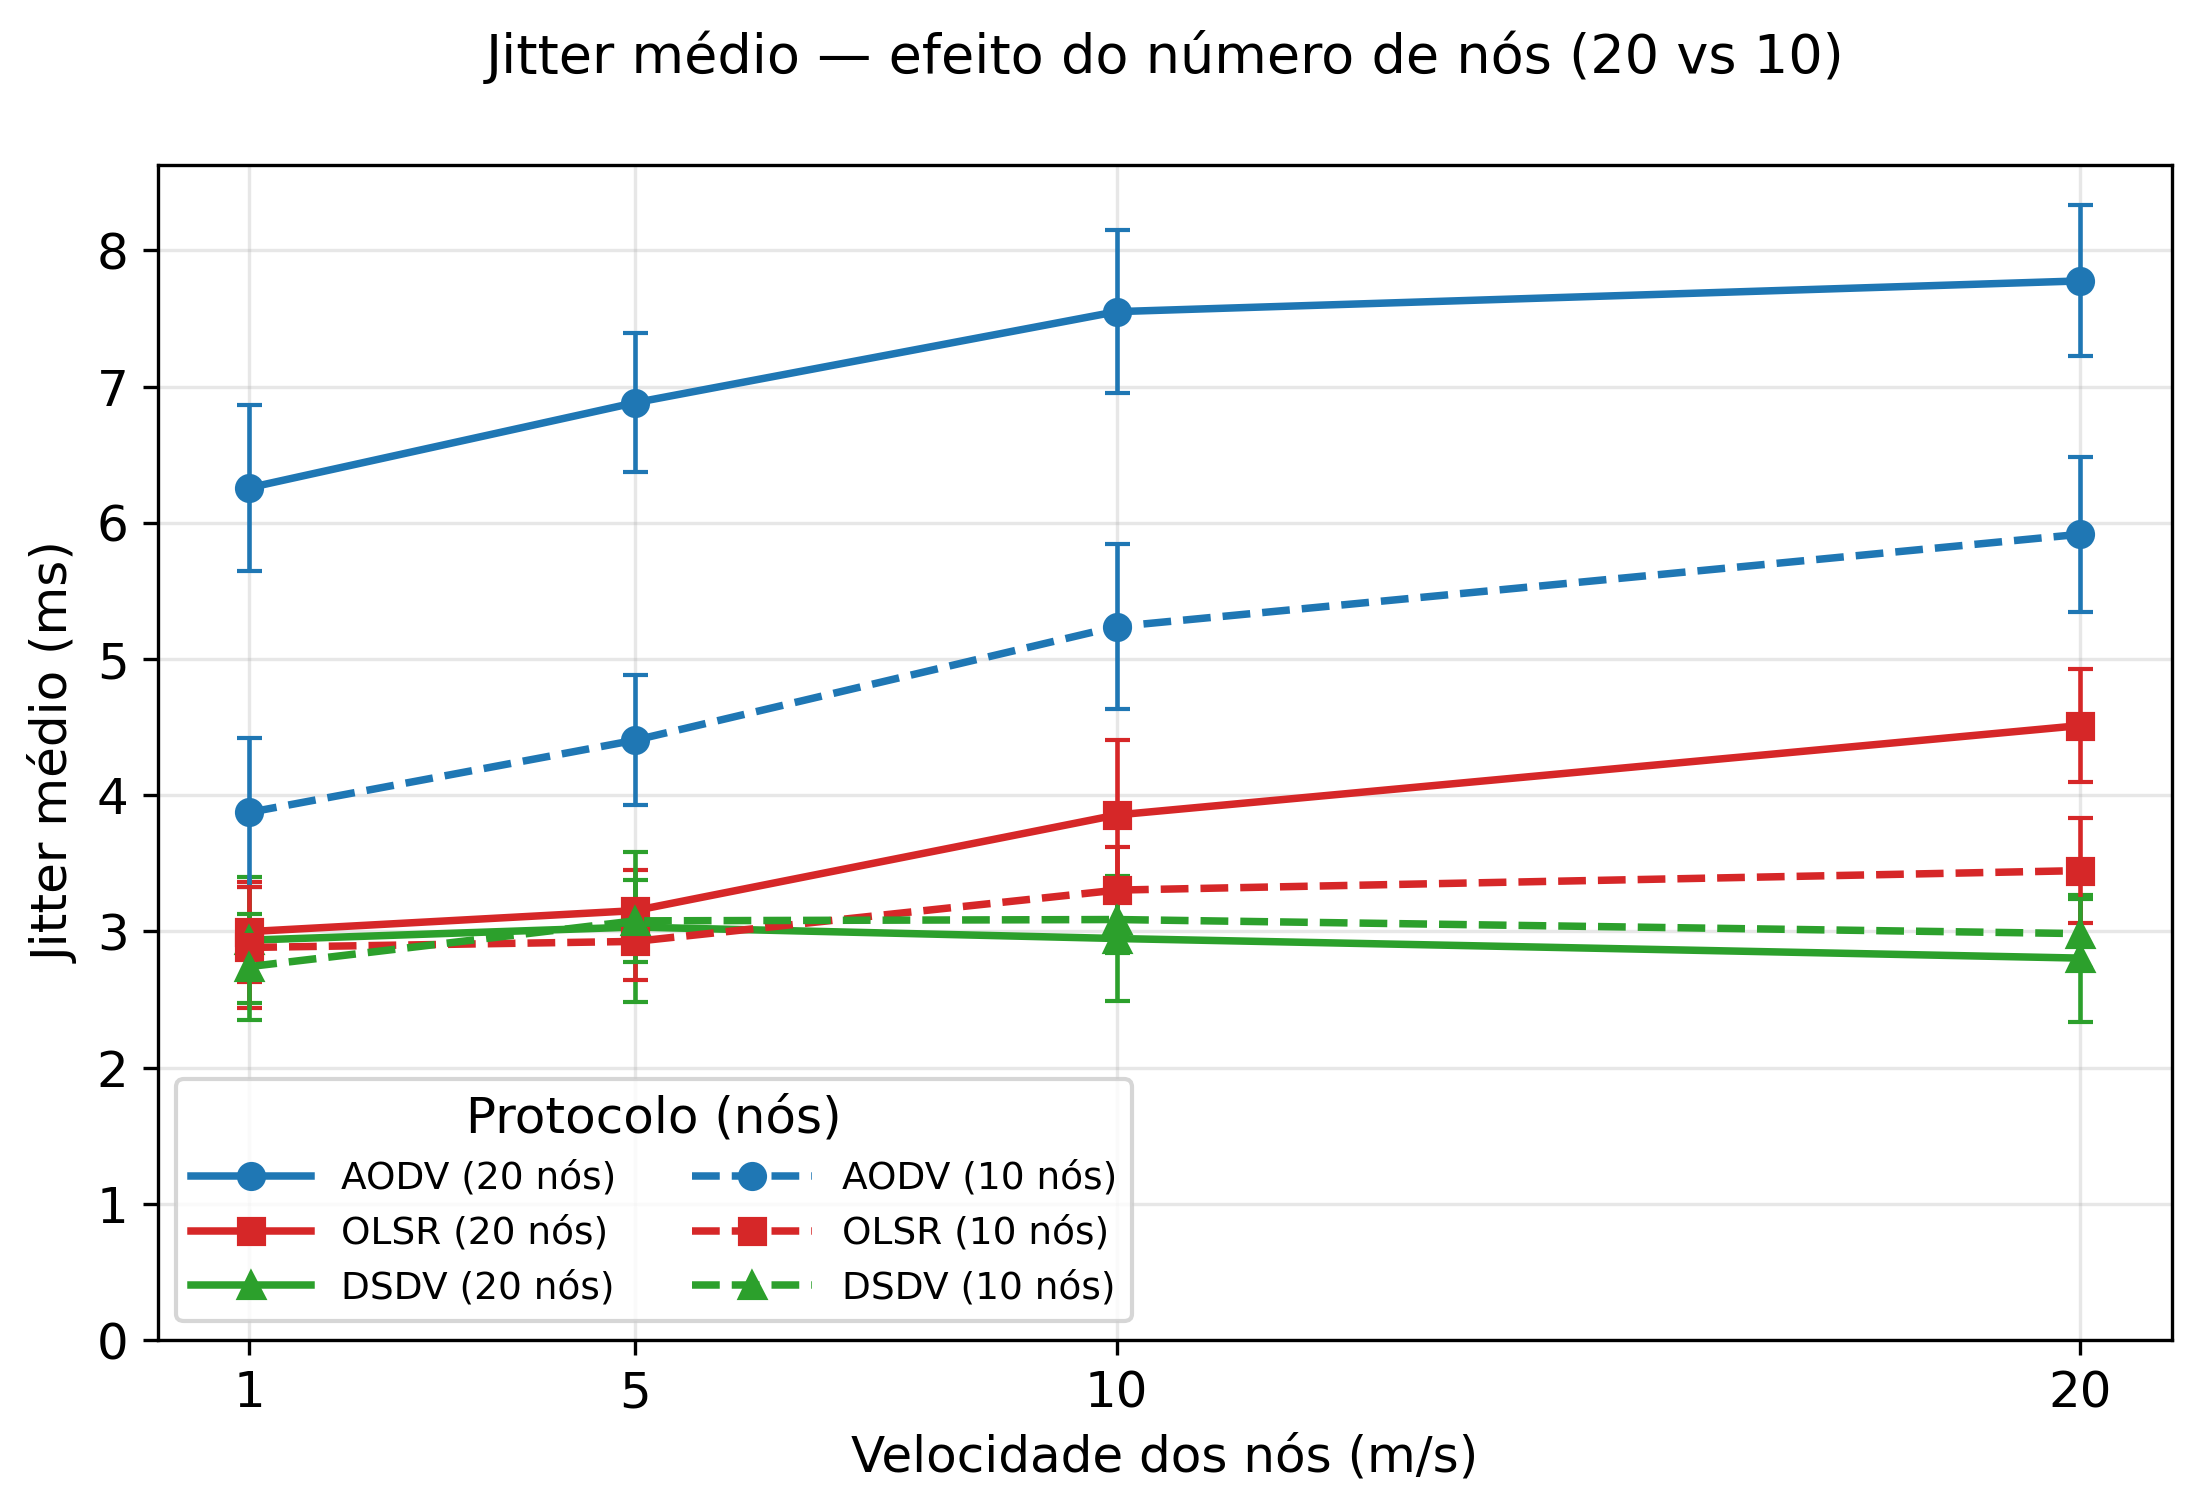
\includegraphics[width=.47\linewidth]{../figures/jitter_nodes_comparison.png}\\[1pt]
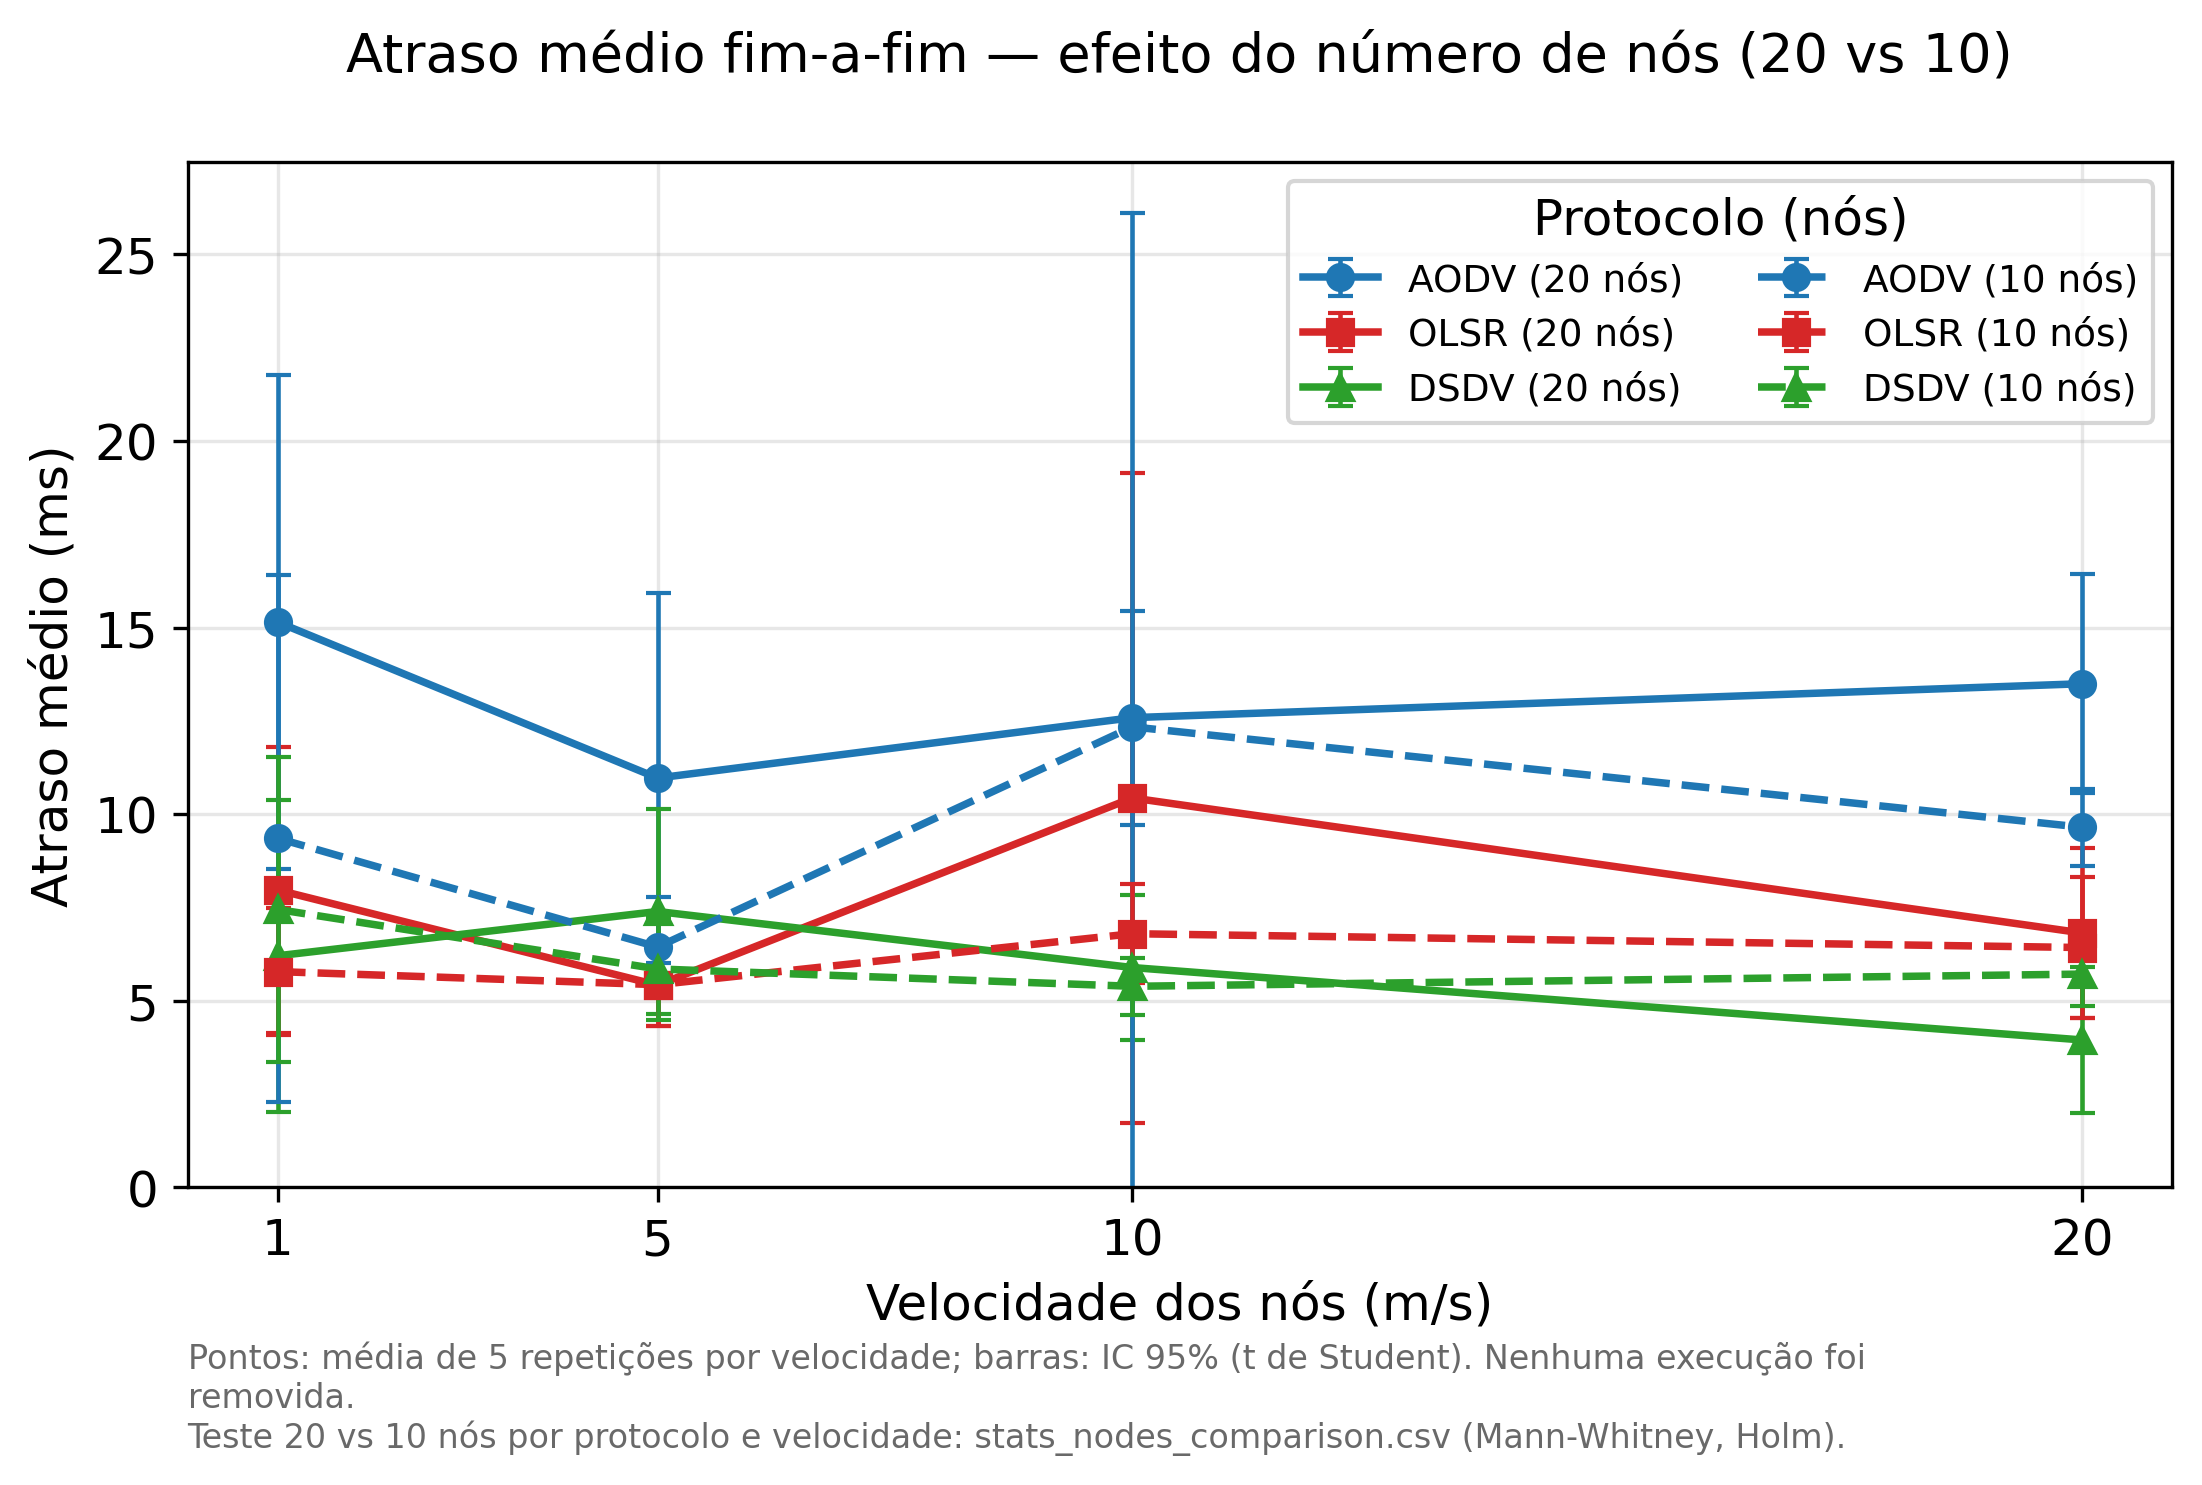
\includegraphics[width=.47\linewidth]{../figures/delay_nodes_comparison.png}
\hfill
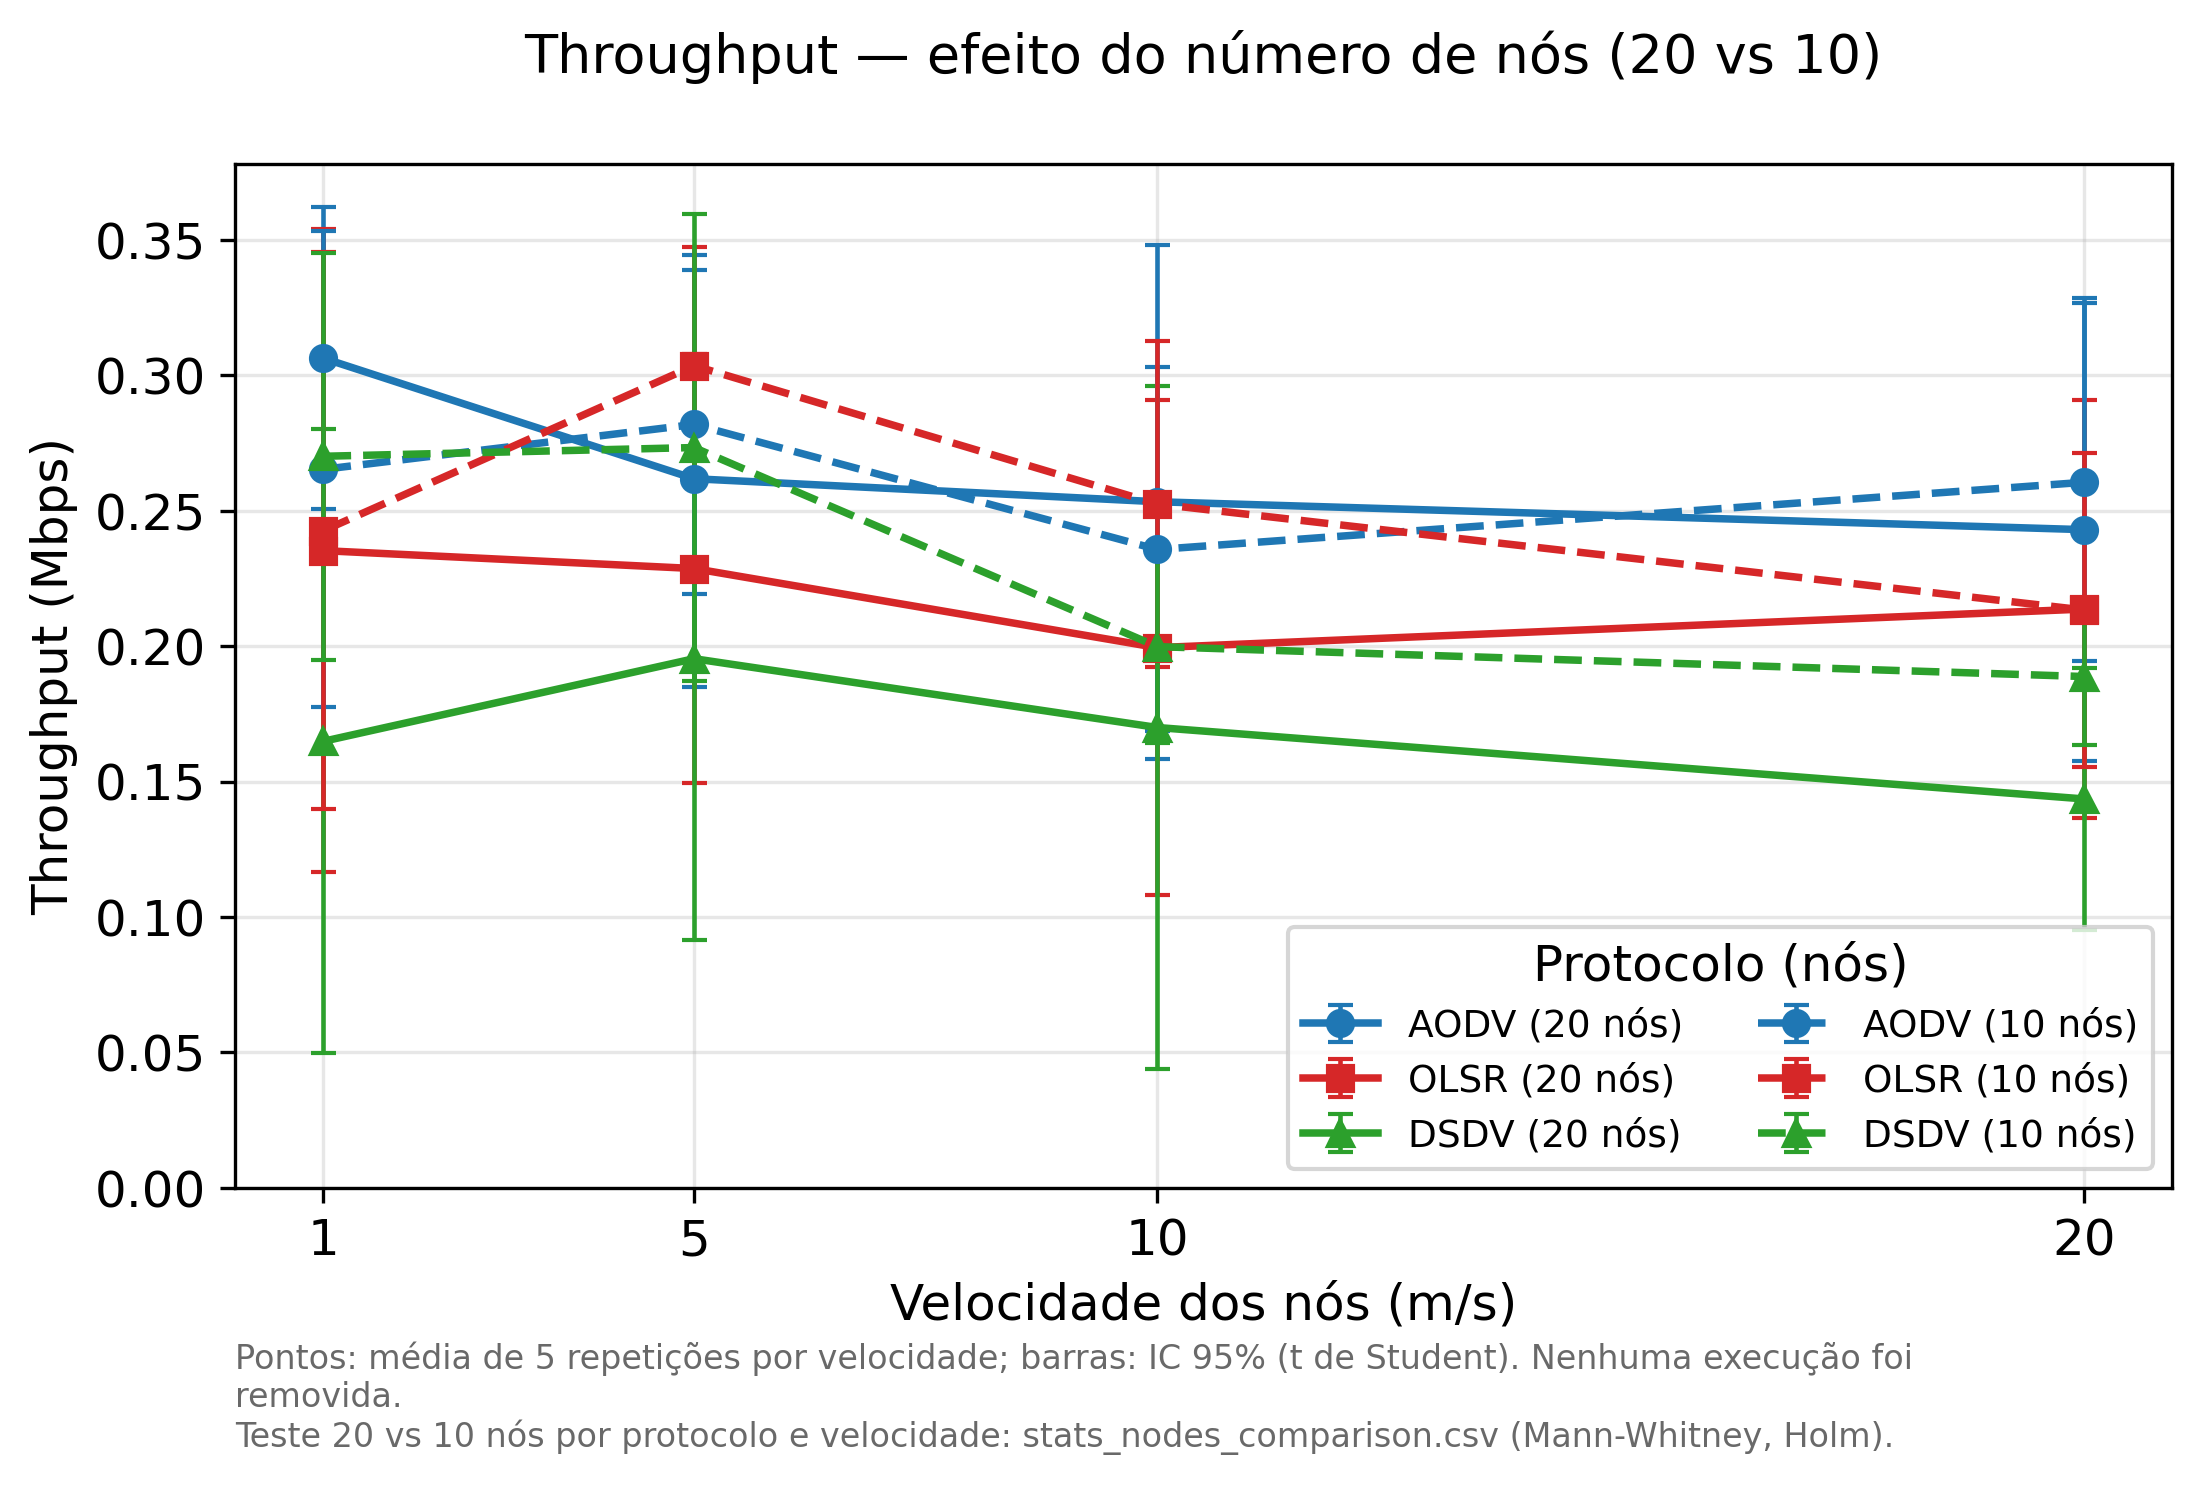
\includegraphics[width=.47\linewidth]{../figures/throughput_nodes_comparison.png}
\caption{PDR, jitter, atraso e throughput: 20 nós (sólido) vs. 10 nós (tracejado).}
\label{fig:pdr-jitter}
\end{figure}

\subsection{Efeito do protocolo}

Com 20 nós, o PDR do AODV só é significativamente maior que o do OLSR a 20~m/s ($p=0{,}003$); nas demais velocidades não há diferença ($p \geq 0{,}23$). Ambos têm PDR significativamente maior que o DSDV em todas as velocidades ($p<0{,}001$). Em atraso e jitter, o AODV é significativamente maior que os outros dois em \emph{todas} as velocidades ($p<0{,}001$, delta de Cliff $\geq 0{,}68$).

Isolando a velocidade: o DSDV é o mais sensível, PDR caindo de 56,9\% (1~m/s) para 43,6\% (20~m/s) -- atualizações periódicas defasam com a topologia mudando rápido. O OLSR é estável até 10~m/s ($\sim$75\%) e só degrada a 20~m/s (66,5\%) -- ponto de degradação concentrado em alta mobilidade. O AODV não cai (73,4\%--76,6\%), mas seu atraso cresce com a velocidade (11,5$\to$13,1~ms); OLSR/DSDV quase não variam (6--8~ms).

A Figura~\ref{fig:aggregate} agrega os três protocolos a 20~m/s.

\begin{figure}[H]
\centering
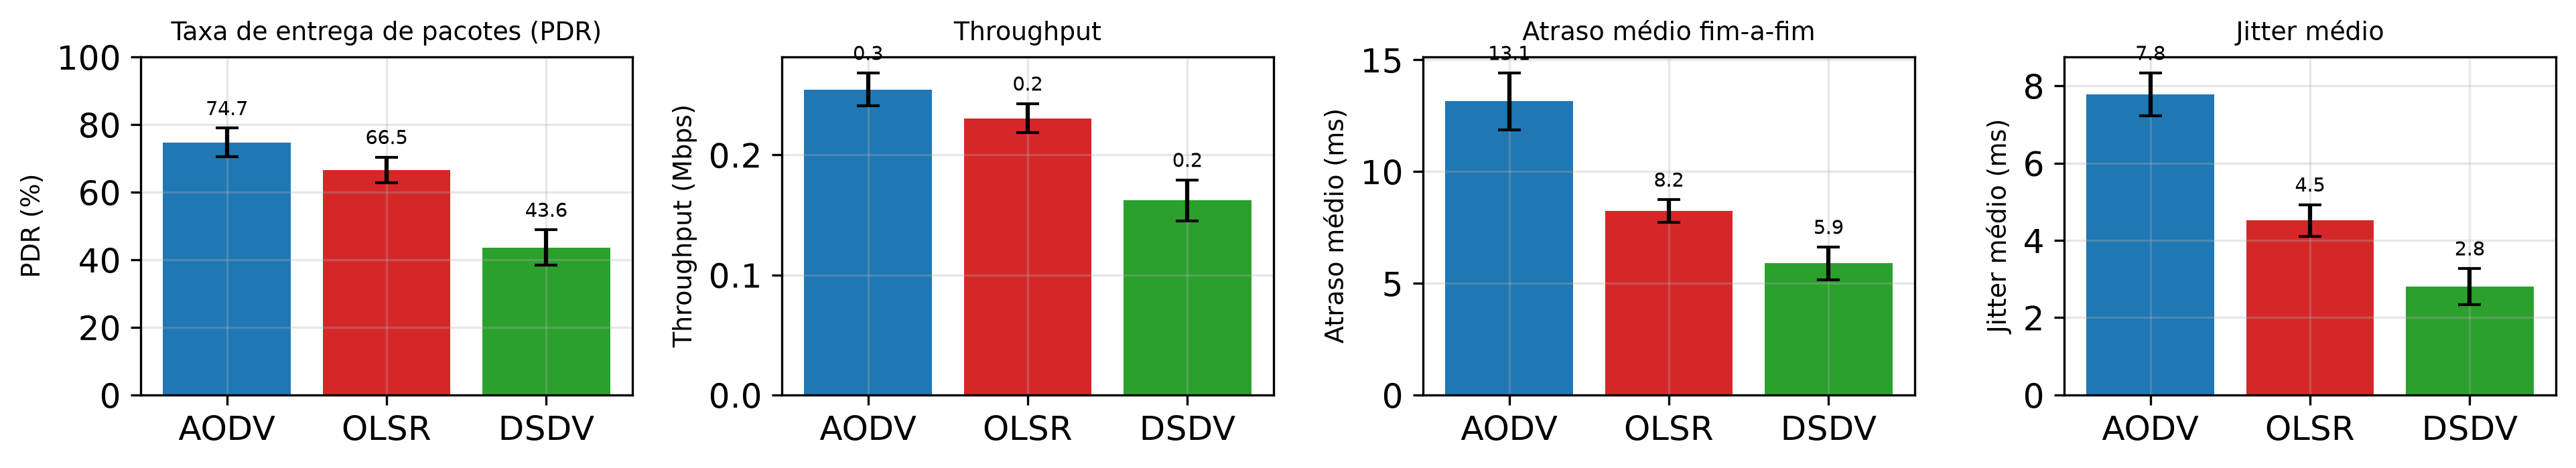
\includegraphics[width=.8\linewidth]{../figures/aggregate_comparison_20n.png}
\caption{Comparação agregada entre AODV, OLSR e DSDV a 20~m/s (20 nós).}
\label{fig:aggregate}
\end{figure}

\vspace{-7mm}
\subsection{Efeito da densidade de nós}
\label{sec:densidade}

A Tabela~\ref{tab:density} resume, por protocolo e métrica, em quantas das 4 velocidades a diferença entre 20 e 10 nós é estatisticamente significativa (Mann-Whitney, correção de Holm). O padrão é marcadamente assimétrico.

\begin{table}[H]
\centering
\caption{Transições 20 vs. 10 nós estatisticamente significativas, de 4 velocidades.}
\label{tab:density}
\footnotesize
\renewcommand{\arraystretch}{0.75}
\begin{tabular}{lcccc}
\hline
\textbf{Protocolo} & \textbf{PDR} & \textbf{Atraso} & \textbf{Jitter} & \textbf{Throughput} \\
\hline
AODV & 0/4 & 2/4 (20n pior) & 4/4 (20n pior) & 0/4 \\
OLSR & 0/4 & 1/4 (20n pior) & 1/4 (20n pior) & 0/4 \\
DSDV & 4/4 (10n melhor) & 0/4 & 0/4 & 4/4 (10n melhor) \\
\hline
\end{tabular}
\end{table}

O DSDV tem PDR e throughput \emph{significativamente maiores} com 10 nós, nas 4 velocidades -- oposto à intuição de que menos nós deveria sempre piorar a rede. O AODV é o inverso: PDR/throughput não mudam com a densidade, mas jitter é maior com 20 nós em todas as velocidades, e atraso a 1 e 5~m/s. O OLSR só sofre em alta mobilidade (20~m/s).

\vspace{3mm}
\section{Discussão}
\label{sec:discussao}

O resultado central é duplo. Primeiro, o AODV não é uniformemente o ``melhor'' protocolo: empata com o OLSR em PDR na maior parte das velocidades, mas perde em atraso e jitter. Segundo, e menos óbvio, reduzir a densidade de nós não prejudica a rede uniformemente -- melhora o DSDV, piora o AODV, e quase não afeta o OLSR.

A assimetria entre protocolos vem do comportamento interno de cada um. O AODV enfileira pacotes enquanto descobre uma rota (RREQ/RREP) e os entrega atrasados; OLSR e DSDV descartam o pacote se não há rota válida no envio. Como atraso e jitter só contam pacotes recebidos, os pacotes ``recuperados'' pelo AODV entram na média com atraso alto, enquanto em OLSR/DSDV eles só reduzem o PDR.

O efeito da densidade liga-se ao mecanismo de cada protocolo. O DSDV retransmite periodicamente a tabela \emph{inteira}: mais nós, broadcasts maiores e mais colisões -- 20 nós prejudica o mecanismo que deveria dar redundância. O AODV inunda a rede com RREQ sob demanda: mais nós, mais retransmissores e saltos, então a fila cresce com a densidade mesmo a entrega não mudando. O OLSR, com retransmissores multiponto \cite{alzahrani2020}, é o mais resistente -- só sofre com mobilidade alta e mais nós juntos.

Isso converge com \cite{alkhatib2018} (proativo igualando/superando reativos sob certas topologias) e qualifica a conclusão mais comum de reativos superarem proativos em geral \cite{quadri2025,arunkumar2008,shrivastava2021}: a resposta depende de qual variável -- velocidade ou densidade -- está em jogo, não só da classe do protocolo.

\vspace{3mm}
\section{Conclusão}

Com 60 repetições e testes não paramétricos, mostramos dois resultados que contestam suposições comuns: a superioridade do AODV sobre proativos não se sustenta em PDR contra o OLSR (só contra o DSDV); e reduzir a densidade de nós não prejudica a rede uniformemente -- melhora o DSDV, piora o AODV e quase não afeta o OLSR, cada um por um mecanismo diferente. Corrigimos ainda um problema de reprodutibilidade nos fluxos de números aleatórios do simulador. Trabalhos futuros: estender ao DSR e medir o overhead de controle por protocolo e densidade.

\vspace{3mm}
\bibliographystyle{sbc}
\bibliography{referencias}

\end{document}
